\documentclass[12pt,a4paper]{article}

\usepackage{mathtools}
\usepackage{graphicx}
\DeclarePairedDelimiter\bra{\langle}{\rvert}
\DeclarePairedDelimiter\ket{\lvert}{\rangle}
\DeclarePairedDelimiterX\braket[2]{\langle}{\rangle}{#1 \delimsize\vert #2}

\usepackage{amsthm}

\usepackage{lmodern} % police européennes  vectorielles  CM
\usepackage[utf8]{inputenc} % encodage à privilégier pour la  portabilité et +
\usepackage[frenchb]{babel} % francisation  de  libellés et de la typographie
\usepackage[T1]{fontenc} % encodage européen des caractères (Cork)8



\newtheorem{definition}{Définition}
\newtheorem{pb}{Problème}
\newtheorem{rem}{Remarque}
\newtheorem{ex}{Exemple}

\title{Algorithme de Deutsch-Jozsa}
\date{}


\begin{document}
\maketitle

\section{Problème à résoudre}
Soit une fonction $f$ booléenne définie par 
\[
  \begin{array}{llll}
    f :  &  \{0, 1\}^n              & \to       & \{ 0, 1 \} \\
         &  (x_0, x_1, \dots , x_n) & \mapsto   &  y = f(x_0, x_1, \dots , x_n), 
  \end{array}  
\]

\begin{definition}
  Une fonction booléenne $f$ est dite équilibrée si $f$ retourne 0
  pour la moitié de ses entrées.
\end{definition}

\begin{definition}
  Une fonction est dite constante si elle retourne une constante pour
  toutes ses entrées.
\end{definition}


\begin{rem}
  Avec $n$ un entier et comme les fonctions booléennes sont à valeur
  dans $\{0,1\}$, il n'existe que deux fonctions constantes $f_0$ et
  $f_1$.
\end{rem}

\begin{ex}
  Soit $f$ la fonction booléenne $f : \{0,1\}^2 \to \{0,1\}$ définie
  par la table de vérité suivante :
\[
  \begin{array}{|c|c|}
    \hline
   (x_1, x_2) & f(x_1,x_2) \\
    \hline
    (0,0) & 0 \\
    \hline
    (0,1) & 1 \\
    \hline
    (1,0) & 1 \\
    \hline
    (1,1) & 0 \\
    \hline
  \end{array}
\]
Cette fonction est équilibrée. On notera qu'elle correspond au
classique ``ou exclusif''. Cette fonction pourrait être représentée
par le vecteur de ces valeurs : $(0,1,1,0)$. Elle peut aussi être
codée en listant les emplacements où elle est vraie, ici $\{1,2\}$.
\end{ex}

\begin{rem}
  Dénombrer les fonctions équilibrées revient à dénombrer les façons
  de placer le symbole le symbole $1$ dans la moitié des cases d'un
  vecteur de taille $2^n$. Avec les emplacements, cela revient à
  dénombrer l'ensemble de sous-ensembles de $\{0, \dots, 2^{n}-1 \}$
  qui ont pour cardinal $2^n / 2$. Finalement, il a donc
  ${\displaystyle {2^n \choose 2^{n-1}}}$ fonctions équilibrées. Ce qui fait
  \[ {\displaystyle {2^n \choose 2^{n-1}}} = \frac{(2^n)!}{(2^{n-1})!(2^n-2^{n-1})!} = \frac{(2^n)!}{((2^{n-1})!)^2}.  \]

  On notera que la proportion des fonctions équilibrées sur l'ensemble
  des $2^{2^n}$ fonctions booléennes de $n$ variables diminue très
  rapidement avec $n$.
  
\end{rem}


\begin{pb}[Deutsch-Jozsa]
Etant donnée une fonction $f$ qui est soit équilibrée, soit constante.
Le problème de Deutsch-Jozsa est de déterminer si $f$ est constante ou
non.  
\end{pb}

\subsection{Solution classique}
Dans le cas classique, il faut effectuer au pire $2^{n-1}+1$
évaluations pour déterminer si $f$ est constante ou équilibrée. Tout
d'abord, dès que deux évaluations sont différentes, $f$ est
nécessairement équilibrée. De plus, si après avoir évalué $2^{n-1}$
entrées et obtenu la même valeur, une évaluation supplémentaire nous
permet de connaitre dans quelle catégorie $f$ se trouve.

\subsection{Solution quantique}
Dans le cas quantique, ce problème se résout en une seule évaluation
quantique de $f$.

\begin{figure}[htbp]
    \centering
    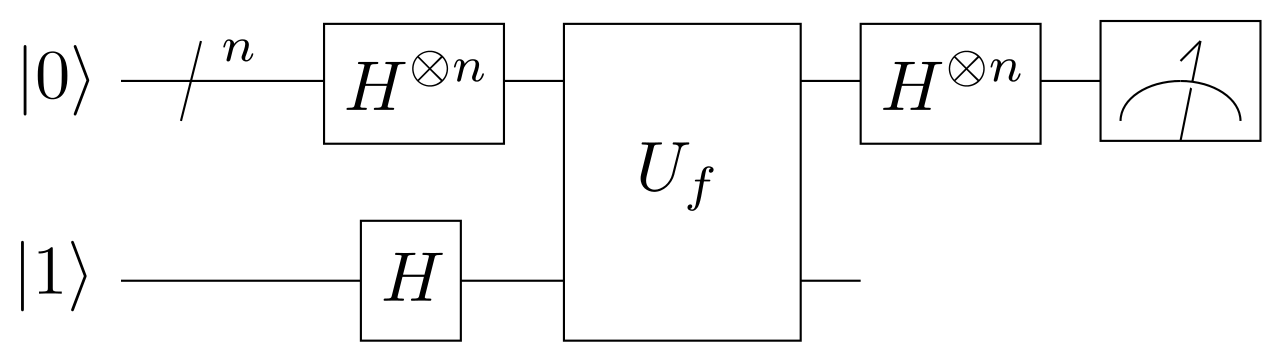
\includegraphics[scale=0.2]{Deutsch-Jozsa_Algorithm.png}
    \caption{Schéma de l'algorithme}
    \label{fig:univerise}
\end{figure}

\subsubsection{Initialisation}
On commence avec :
$\ket{u_0} = (\ket{0}^{\bigotimes n}) \otimes \ket{1}$
: n-qubits à $\ket{0}$ et 1-qubit à $\ket{1}$

\subsubsection{Etape 1}

On applique une porte de Hadamard à $\ket{u_0}$ pour avoir un état équiprobable:
$\ket{u_1} = H\ket{u_0} = \frac{1}{\sqrt{2^{n + 1}}}
\displaystyle\sum_{x=0}^{2^n-1} \ket{x}(\ket{0} - \ket{1})$

\subsubsection{Etape 2}
On applique l'oracle quantique suivant à $\ket{u_1}$:
\[ o : \ket{x}\ket{y}\mapsto \ket{x}\ket{y\oplus f(x)}. \]

Posons $x$, on est alors dans l'une des deux situations disjointes suivantes :
\begin{itemize}
\item $f(x) = 0$,
\item $f(1) = 0$.
\end{itemize}

Analysons chacune de ces situations, tout d'abord si $f(x) = 0$ alors
%Prenons le cas à 1 qubit:
\[
o : \ket{x}(\ket{0} - \ket{1}) \mapsto \ket{x}(\ket{0} - \ket{1})
\]
Autrement dit $\ket{x}(\ket{0} - \ket{1}$ est un  point fixe de $o$.

Dans l'autre situation, on a $f(x) = 1$ et on en déduit
\[
o : \ket{x}(\ket{0} - \ket{1}) \mapsto \ket{x}(\ket{1} - \ket{0})
\]
Autrement dit, dans ce cas, le vecteur $\ket{x}(\ket{0} - \ket{1})$
est envoyé sur son opposé via $o$.

Finalement, les deux cas précédents peuvent être résumé sous la forme suivante
\[
o : \ket{x}(\ket{0} - \ket{1}) \mapsto (-1)^{f(x)}\ket{x}(\ket{0} - \ket{1})
\]

Par linéarité, on en déduit :

\begin{equation}\ket{u_2} = \frac{1}{\sqrt{2^{n + 1}}} 
\displaystyle\sum_{x=0}^{2^n-1} (-1)^{f(x)}\ket{x}(\ket{0} - \ket{1}) 
\end{equation}

On peut ignorer le dernier qubit ($\ket{0} - \ket{1}$) comme il est
constant. Finalement, on en déduit :
\begin{equation}
\ket{u_2} = \frac{1}{\sqrt{2^{n + 1}}}
\displaystyle\sum_{x=0}^{2^n-1} (-1)^{f(x)}\ket{x}
\end{equation}

\subsubsection{Etape 3}

Maintenant qu'on a appliqué notre oracle, on est toujours dans un état
"probabiliste", et en mesurant nous n'obtiendrons pas une réponse
exacte à notre problème. L'objectif est donc maintenant de ramener les
solutions sur un état déterminé pour obtenir la réponse
systématique. En appliquant la porte de Hadamard, on va pouvoir forcer
un état à apparaître pour un type de fonction $f$, et le forcer à
disparaître dans l'autre cas, ce qui nous permet d'avoir une réponse
systématique sur le type de la fonction : est-elle équilibrée ou bien constante ?

On réapplique une porte Hadamard à chaque qubit sortant, ce qui donne:

\[ \ket{u_3} = \frac{1}{\sqrt{2^{n}}}
\displaystyle\sum_{x=0}^{2^n-1} (-1)^{f(x)} \left( \frac{1}{\sqrt{2^{n}}} \displaystyle\sum_{y=0}^{2^n-1} (-1)^{x.y}\ket{y} \right) \]

Par linéarité, on a :
\begin{equation}
  \label{eq:1}
  \ket{u_3} = \frac{1}{2^{n}}
  \displaystyle\sum_{x=0}^{2^n-1} \displaystyle\sum_{y=0}^{2^n-1}(-1)^{f(x)} (-1)^{x.y}\ket{y}  
\end{equation}

La probabilité $|p|$ de mesurer $\ket{0}^{\bigotimes n}$ est donc : 
\begin{equation}
  \label{eq:2}
  |\frac{1}{2^{n}}\displaystyle\sum_{x=0}^{2^n-1}(-1)^{f(x)}|
\end{equation}

avec $p = \frac{1}{2^{n}}\displaystyle\sum_{x=0}^{2^n-1}(-1)^{f(x)}$.

Si on a une fonction $f(x)$ constante, alors chaque élément de la
somme retourne la même valeur (1 ou -1 suivant que $f(x)$ retourne 0
ou 1), la somme va donc valoir $\pm 2^{n}$. Dans le cas où la fonction
est équilibrée, on va avoir autant de 1 que de -1, la somme est donc
nulle.

On a donc les valeurs suivantes dépendant du type de $f(x)$ :
\begin{enumerate}
  \item Si $f(x)$ est constante :  $p = \pm \frac{1}{2^n} \times 2^{n} = \pm 1$,
  \item Si $f(x)$ est équilibrée : $p = \pm \frac{1}{2^n} \times 0 = 0$.
\end{enumerate}

Dans le cas constant, on ne peut donc que mesurer $\ket{0}^{\bigotimes n}$ puisqu'il a une probabilité de 1 d'apparaître. Dans le cas équilibré, on ne mesure jamais $\ket{0}^{\bigotimes n}$ puisque sa probabilité est nulle.

On en conclut que, lorsqu'on effectue une mesure, si on tombe sur $\ket{0}^{\bigotimes n}$ alors la fonction est constante, sinon elle est équilibrée.

%'objectif de cette dernière étape est de passer 

\subsection{Exemple}

Prenons une fonction $f$ comme définie précédemment avec $n=2$, sans
savoir si elle est constante ou équilibrée.

\subsubsection{Etape 1}


On commence avec $\ket{u_0} = \ket{001}$. La première étape est
l'application de la porte d'hadamard à $\ket{u_0}$:

\begin{align}
\ket{u_1} &= H\ket{u_0} = H\ket{0} \otimes H\ket{0} \otimes H\ket{1} \\
& = \frac{1}{2\sqrt{2}} \left( (\ket{0} + \ket{1})\otimes(\ket{0} + \ket{1})\otimes(\ket{0} - \ket{1}) \right) \\
 & = \frac{1}{2\sqrt{2}}\{\ket{000} - \ket{001} + \ket{010} - \ket{011} + \ket{100} - \ket{101} + \ket{110} - \ket{111}\} \\
& = \frac{1}{2\sqrt{2}}\{\ket{00}(\ket{0} - \ket{1}) + \ket{01}(\ket{0} - \ket{1}) + \ket{10}(\ket{0} - \ket{1}) + \ket{11}(\ket{0} - \ket{1})\}
\end{align}

%On peut factoriser le tout par $(\ket{0} - \ket{1})$: 
%$

\subsubsection{Etape 2: oracle quantique}

On applique à $\ket{u_1}$ l'oracle quantique $\ket{x}\ket{y}\rightarrow\ket{x}\ket{y\oplus f(x)}:$

\begin{align*}
\ket{u_2}  =  \frac{1}{2\sqrt{2}}  & \ket{00}(\ket{0 \oplus f(00)} - \ket{1 \oplus f(00)}) + \\
& \ket{01}(\ket{0 \oplus f(01)} - \ket{1 \oplus f(01)}) + \\
& \ket{10}(\ket{0 \oplus f(10)} - \ket{1 \oplus f(10)}) + \\
& \ket{11}(\ket{0 \oplus f(11)} - \ket{1 \oplus f(11)})  \\
\end{align*}


On peut alors réécrire l'équation de la façon suivante: 



\begin{align*}
  \ket{u_2} = \frac{1}{2\sqrt{2}} & (-1)^{f(00)} \ket{00}  (\ket{0} - \ket{1}) + \\
&(-1)^{f(01)} \ket{01}  (\ket{0} - \ket{1}) + \\
&(-1)^{f(10)} \ket{10}  (\ket{0} - \ket{1}) + \\
&(-1)^{f(11)} \ket{11}  (\ket{0} - \ket{1}) 
\end{align*}

Par la suite, on va appliquer une porte de Hadamard à $\ket{u_2}$. Le qubit $\ket{0} - \ket{1}$ donne $\ket{1}$ par la cette porte, il est donc constant par rapport à $\ket{u_0}$. On peut donc le retirer de l'équation, ce qui nous donne pour $\ket{u_2}$ :

\begin{equation}
  \label{eq:3}
\ket{u_2} = \frac{1}{2\sqrt{2}} \left( (-1)^{f(00)} \ket{00} + (-1)^{f(01)} \ket{01} + (-1)^{f(10)} \ket{10} + (-1)^{f(11)} \ket{11} \right) 
\end{equation}


Matriciellement, on peut donc écrire

\begin{equation}
  \label{eq:4}
\ket{u_2} = \left(  \begin{array}{cccc}
     (-1)^{f(00)}  &0 & 0 &0 \\
     0 & (-1)^{f(01)} & 0 &0 \\
     0 &0 & (-1)^{f(10)} &0 \\
     0 &0 & 0 & (-1)^{f(11)} \\
        \end{array}
      \right)
      \left(  \begin{array}{c}
                1 \\
                1 \\
                1 \\
                1 
              \end{array}
      \right)      
\end{equation}


\subsubsection{Etape 3: porte de Hadamard}

On applique donc une porte de hadamard à $\ket{u_2}$:
\begin{equation}
  \label{eq:5}
\ket{u_3} = \frac{1}{2\sqrt{2}} H \left( (-1)^{f(00)} \ket{00} + (-1)^{f(01)} \ket{01} + (-1)^{f(10)} \ket{10} + (-1)^{f(11)} \ket{11} \right) 
\end{equation}

Nous sommes sur une porte de hadamard pour 2 qubits, ce qui donne
la relation matricielle suivante pour $\ket{u_3}$:

\begin{align}
\ket{u_3} &=
\frac{1}{4\sqrt{2}} 
\begin{bmatrix}
  1 & 1 & 1 & 1 \\
  1 & -1 & 1 & -1 \\
  1 & 1 & -1 & -1 \\
  1 & -1 & -1 & 1 \\
\end{bmatrix}
\begin{bmatrix}
  (-1)^{f(00)} \\ (-1)^{f(01)} \\ (-1)^{f(10)} \\ (-1)^{f(11)}
\end{bmatrix} , \\ 
 &= \frac{1}{4\sqrt{2}} 
\begin{bmatrix}
  (-1)^{f(00)} + (-1)^{f(01)} + (-1)^{f(10)} + (-1)^{f(11)} \\
  (-1)^{f(00)} - (-1)^{f(01)} + (-1)^{f(10)} - (-1)^{f(11)} \\
  (-1)^{f(00)} + (-1)^{f(01)} - (-1)^{f(10)} - (-1)^{f(11)} \\
  (-1)^{f(00)} - (-1)^{f(01)} - (-1)^{f(10)} + (-1)^{f(11)} \\
\end{bmatrix}.
\end{align}

Si f est constante , alors
$(-1)^{f(00)} = (-1)^{f(01)} = (-1)^{f(10)} = (-1)^{f(11)}$. En
fonction du fait que $f=0$ ou bien $f=1$:

\begin{equation}
  \label{eq:6}
\ket{u_3}=
\frac{1}{\sqrt{2}} 
\begin{bmatrix}
  1 \\ 0 \\ 0 \\ 0
\end{bmatrix}  \text{ ou bien }
\ket{u_3}=
\frac{1}{\sqrt{2}} 
\begin{bmatrix}
  -1 \\ 0 \\ 0 \\ 0
\end{bmatrix}.
\end{equation}
On a donc une probabilité de $1$ de mesurer l'état $\ket{00}$.


En revanche, si f est équilibrée, la moitié des valeurs vont
valoir $(-1)^{0} = 1$ et l'autre moitié $(-1)^{1} = -1$. La première
ligne du vecteur $\ket{u_3}$ donne donc systématiquement 0, on ne mesure donc
jamais l'état $\ket{00}$.

\medbreak

\end{document}

%%% Local Variables:
%%% mode: latex
%%% TeX-master: t
%%% End:
